%%%%%%%%%%%%%%%%%%%%%%%%%%%%%%%%%%%%%%%%%
% Beamer Presentation
% LaTeX Template
% Version 2.0 (March 8, 2022)
%
% This template originates from:
% https://www.LaTeXTemplates.com
%
% Author:
% Vel (vel@latextemplates.com)
%
% License:
% CC BY-NC-SA 4.0 (https://creativecommons.org/licenses/by-nc-sa/4.0/)
%
%%%%%%%%%%%%%%%%%%%%%%%%%%%%%%%%%%%%%%%%%

%----------------------------------------------------------------------------------------
%	PACKAGES AND OTHER DOCUMENT CONFIGURATIONS
%----------------------------------------------------------------------------------------

\documentclass[
	11pt, % Set the default font size, options include: 8pt, 9pt, 10pt, 11pt, 12pt, 14pt, 17pt, 20pt
	%t, % Uncomment to vertically align all slide content to the top of the slide, rather than the default centered
	%aspectratio=169, % Uncomment to set the aspect ratio to a 16:9 ratio which matches the aspect ratio of 1080p and 4K screens and projectors
]{beamer}

\graphicspath{{Images/}{./}} % Specifies where to look for included images (trailing slash required)

\usepackage{booktabs} % Allows the use of \toprule, \midrule and \bottomrule for better rules in tables
\usepackage{cite}
\usepackage{amsmath,amssymb,amsfonts}

%\usepackage{graphicx}
\usepackage{textcomp}
\usepackage{xcolor}
\usepackage{tikz}
\usepackage{pgfplots}
\usepackage{pgfplotstable}
\usepackage{rtsched}
\usepackage{threeparttable}
\usepackage{csvsimple}
\usepackage{booktabs} % For \toprule, \midrule and \bottomrule
\usepackage{siunitx} % Formats the units and values
%\usepackage[hidelinks]{hyperref}
\usetikzlibrary{patterns,calc,arrows}
\usepackage[utf8]{inputenc}
\usepackage[T1]{fontenc}
\usepackage{pgf}
\usepackage{amsmath}
\usepackage{bm}
\usepackage{url}
%\usepackage{algorithm}
%\usepackage{algpseudocode}
\def\UrlBreaks{\do\/\do-}
\usepackage{breakurl}
%\usepackage[breaklinks,hidelinks]{hyperref}
%----------------------------------------------------------------------------------------
%	SELECT LAYOUT THEME
%----------------------------------------------------------------------------------------

% Beamer comes with a number of default layout themes which change the colors and layouts of slides. Below is a list of all themes available, uncomment each in turn to see what they look like.

%\usetheme{default}
%\usetheme{AnnArbor}
%\usetheme{Antibes}
%\usetheme{Bergen}
%\usetheme{Berkeley}
%\usetheme{Berlin}
%\usetheme{Boadilla}
%\usetheme{CambridgeUS}
%\usetheme{Copenhagen}
%\usetheme{Darmstadt}
%\usetheme{Dresden}
%\usetheme{Frankfurt}
%\usetheme{Goettingen}
%\usetheme{Hannover}
%\usetheme{Ilmenau}
%\usetheme{JuanLesPins}
%\usetheme{Luebeck}
\usetheme{Madrid}
%\usetheme{Malmoe}
%\usetheme{Marburg}
%\usetheme{Montpellier}
%\usetheme{PaloAlto}
%\usetheme{Pittsburgh}
%\usetheme{Rochester}
%\usetheme{Singapore}
%\usetheme{Szeged}
%\usetheme{Warsaw}

%----------------------------------------------------------------------------------------
%	SELECT COLOR THEME
%----------------------------------------------------------------------------------------

% Beamer comes with a number of color themes that can be applied to any layout theme to change its colors. Uncomment each of these in turn to see how they change the colors of your selected layout theme.

%\usecolortheme{albatross}
%\usecolortheme{beaver}
%\usecolortheme{beetle}
%\usecolortheme{crane}
%\usecolortheme{dolphin}
%\usecolortheme{dove}
%\usecolortheme{fly}
%\usecolortheme{lily}
%\usecolortheme{monarca}
%\usecolortheme{seagull}
%\usecolortheme{seahorse}
%\usecolortheme{spruce}
%\usecolortheme{whale}
%\usecolortheme{wolverine}

%----------------------------------------------------------------------------------------
%	SELECT FONT THEME & FONTS
%----------------------------------------------------------------------------------------

% Beamer comes with several font themes to easily change the fonts used in various parts of the presentation. Review the comments beside each one to decide if you would like to use it. Note that additional options can be specified for several of these font themes, consult the beamer documentation for more information.

\usefonttheme{default} % Typeset using the default sans serif font
%\usefonttheme{serif} % Typeset using the default serif font (make sure a sans font isn't being set as the default font if you use this option!)
%\usefonttheme{structurebold} % Typeset important structure text (titles, headlines, footlines, sidebar, etc) in bold
%\usefonttheme{structureitalicserif} % Typeset important structure text (titles, headlines, footlines, sidebar, etc) in italic serif
%\usefonttheme{structuresmallcapsserif} % Typeset important structure text (titles, headlines, footlines, sidebar, etc) in small caps serif

%------------------------------------------------

%\usepackage{mathptmx} % Use the Times font for serif text
\usepackage{palatino} % Use the Palatino font for serif text

%\usepackage{helvet} % Use the Helvetica font for sans serif text
\usepackage[default]{opensans} % Use the Open Sans font for sans serif text
%\usepackage[default]{FiraSans} % Use the Fira Sans font for sans serif text
%\usepackage[default]{lato} % Use the Lato font for sans serif text

%----------------------------------------------------------------------------------------
%	SELECT INNER THEME
%----------------------------------------------------------------------------------------

% Inner themes change the styling of internal slide elements, for example: bullet points, blocks, bibliography entries, title pages, theorems, etc. Uncomment each theme in turn to see what changes it makes to your presentation.

%\useinnertheme{default}
\useinnertheme{circles}
%\useinnertheme{rectangles}
%\useinnertheme{rounded}
%\useinnertheme{inmargin}

%----------------------------------------------------------------------------------------
%	SELECT OUTER THEME
%----------------------------------------------------------------------------------------

% Outer themes change the overall layout of slides, such as: header and footer lines, sidebars and slide titles. Uncomment each theme in turn to see what changes it makes to your presentation.

%\useoutertheme{default}
%\useoutertheme{infolines}
%\useoutertheme{miniframes}
%\useoutertheme{smoothbars}
%\useoutertheme{sidebar}
%\useoutertheme{split}
%\useoutertheme{shadow}
%\useoutertheme{tree}
%\useoutertheme{smoothtree}

%\setbeamertemplate{footline} % Uncomment this line to remove the footer line in all slides
%\setbeamertemplate{footline}[page number] % Uncomment this line to replace the footer line in all slides with a simple slide count

%\setbeamertemplate{navigation symbols}{} % Uncomment this line to remove the navigation symbols from the bottom of all slides

%----------------------------------------------------------------------------------------
%	PRESENTATION INFORMATION
%----------------------------------------------------------------------------------------

\title[Short Title]{Energy aware memory allocation in real-time systems} % The short title in the optional parameter appears at the bottom of every slide, the full title in the main parameter is only on the title page

\subtitle{CCM-SRAM allocation to reduce consumption} % Presentation subtitle, remove this command if a subtitle isn't required

\author[]{Loïc Thomas} % Presenter name(s), the optional parameter can contain a shortened version to appear on the bottom of every slide, while the main parameter will appear on the title slide

\institute[UC]{LAAS CNRS \\ \smallskip \textit{lthomas@laas.fr}} % Your institution, the optional parameter can be used for the institution shorthand and will appear on the bottom of every slide after author names, while the required parameter is used on the title slide and can include your email address or additional information on separate lines

\date[\today]{\today} % Presentation date or conference/meeting name, the optional parameter can contain a shortened version to appear on the bottom of every slide, while the required parameter value is output to the title slide

%----------------------------------------------------------------------------------------

\begin{document}

%----------------------------------------------------------------------------------------
%	TITLE SLIDE
%----------------------------------------------------------------------------------------

\begin{frame}
	\titlepage % Output the title slide, automatically created using the text entered in the PRESENTATION INFORMATION block above
\end{frame}

%----------------------------------------------------------------------------------------
%	TABLE OF CONTENTS SLIDE
%----------------------------------------------------------------------------------------

% The table of contents outputs the sections and subsections that appear in your presentation, specified with the standard \section and \subsection commands. You may either display all sections and subsections on one slide with \tableofcontents, or display each section at a time on subsequent slides with \tableofcontents[pausesections]. The latter is useful if you want to step through each section and mention what you will discuss.

%----------------------------------------------------------------------------------------
%	PRESENTATION BODY SLIDES
%----------------------------------------------------------------------------------------

\section{Current measurement with Nucleo LPM01A} % Sections are added in order to organize your presentation into discrete blocks, all sections and subsections are automatically output to the table of contents as an overview of the talk but NOT output in the presentation as separate slides

%------------------------------------------------
\begin{frame}
	\frametitle{Current consumption graphic}
	\begin{figure}
		\centering
        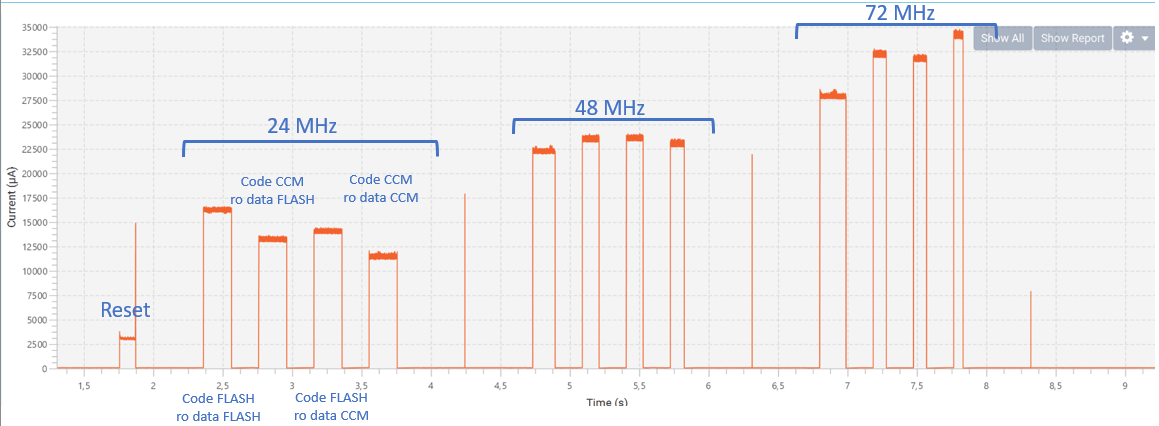
\includegraphics[scale=0.6]{images/pointer_chase_capture_mod.png}
        \caption{Intensity consumption graph for differents pointer chase executions}
	\end{figure}
\end{frame}

%------------------------------------------------
\section{Impact of moving instructions in CCM}
\begin{frame}
	\frametitle{Energy decrease when instruction are moved into CCM}
	\begin{figure}
		\centering
        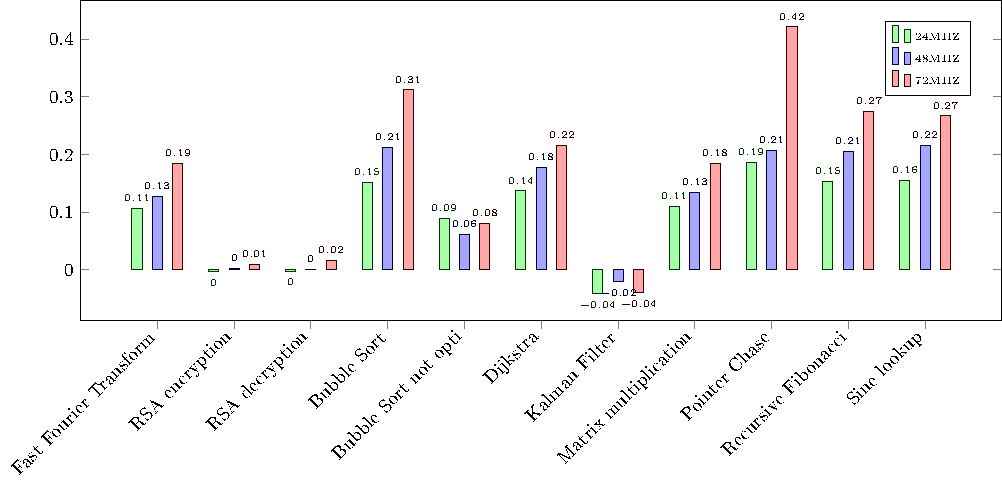
\includegraphics[scale=0.7]{plot/code_ccm_energy.pdf}
	\end{figure}
	Moving instruction into CCM SRAM can overall improve energy consumption 
\end{frame}

\begin{frame}
	\frametitle{Runtime decrease when instruction are moved into CCM}
	\begin{figure}
		\centering
        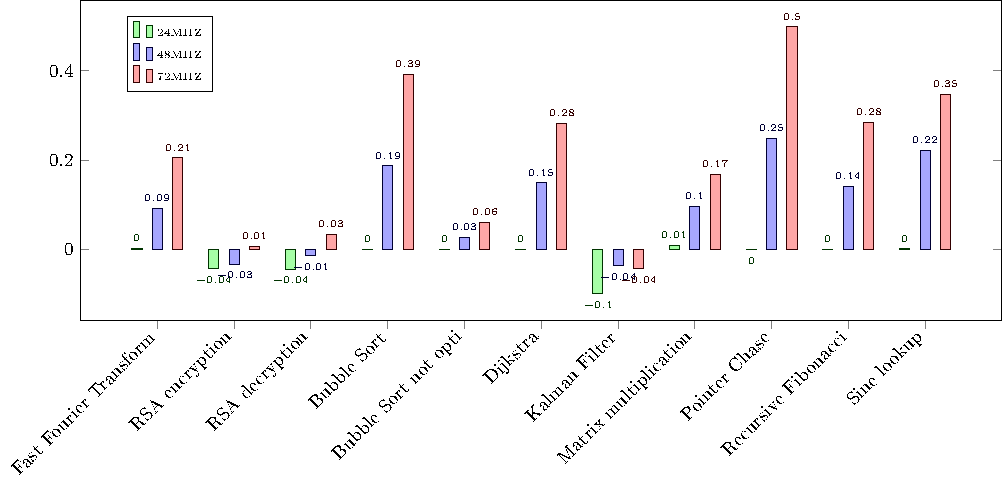
\includegraphics[scale=0.7]{plot/code_ccm_runtime.pdf}
	\end{figure}
	In high frequencies the runtime is reduced when code is moved into CCM SRAM.
\end{frame}

\begin{frame}
	\frametitle{Intensiy decrease when instruction are moved into CCM}
	\begin{figure}
		\centering
        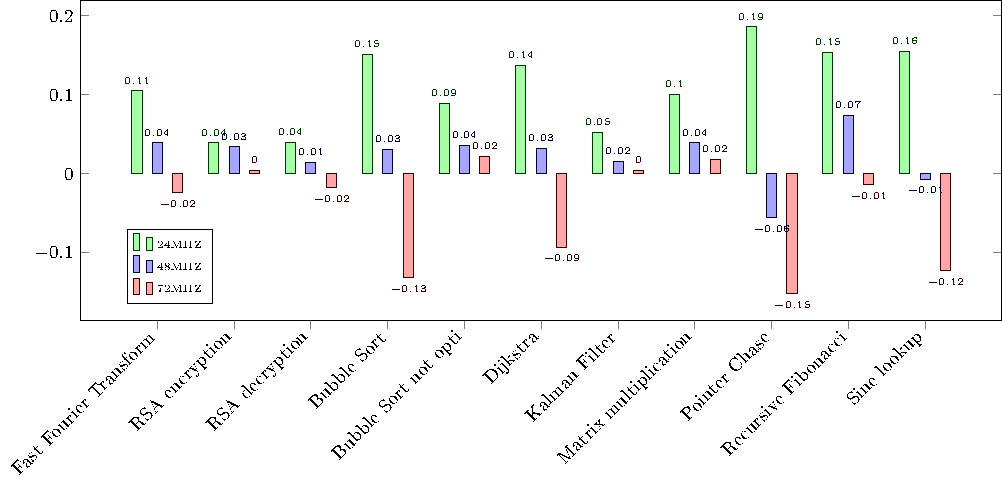
\includegraphics[scale=0.7]{plot/code_ccm_intensity.pdf}
	\end{figure}
	In high frequencies, intensity is lowered when the code is running from flash.
\end{frame}

\begin{frame}
	\frametitle{Wait states impact on intensity}
	\begin{figure}
		\centering
        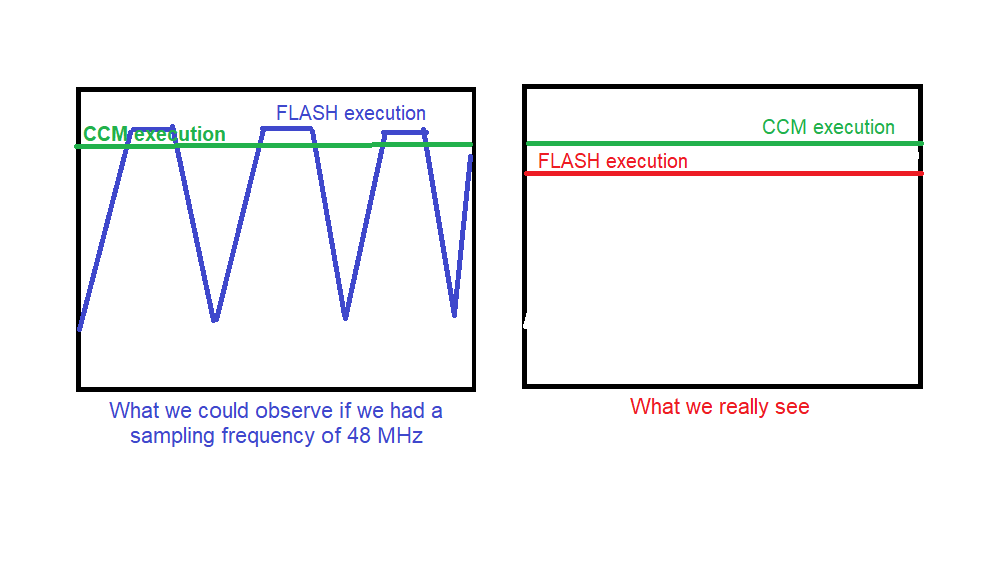
\includegraphics[scale=0.7]{images/wait_state_impact.png}
	\end{figure}
	Wait states lower the average intensity of an execution. 
	This effect is thus increased at high frequency where we have more wait states.
\end{frame}

\section{Energy variation over the frequency}

\begin{frame}
	\frametitle{Absolute energy when code is running from CCM (mJ)}
	
\begin{table}[h!]
\centering
\begin{tabular}{||c c c c||} 
 \hline
 Algorithm & 24MHz & 48MHz & 72MHz \\ [0.5ex] 
 \hline\hline
 Pointer Chase & 8.815 & 9.402 & 10.026 \\ 
 Bubble Sort & 11.294 & 10.962 & 10.893 \\
 Bubble Sort no opti & 43.017 & 42.524 & 41.669 \\
 RSA decrypt & 5.239 & 5.166 & 5.469 \\
 Kalman & 2.301 & 2.357 & 2.665 \\
 Dijkstra & 36.318 & 35.189 & 34.828 \\[1ex] 
 \hline
\end{tabular}
\caption{Absolute energy (mJ) with instruction in CCM SRAM}
\label{energy_tab_code_ccm}
\end{table}

	Energy remains almost the same even if the frequency increases.
\end{frame}

\begin{frame}
	\frametitle{Absolute energy when code is running from FLASH (mJ)}
	\begin{table}[!ht]
    \centering
    \begin{tabular}{||c c c c||}
    \hline
        ~ & 24MHz & 48MHz & 72MHz \\[0.5ex]  \hline \hline
        FFT & 0.293 & 0.292 & 0.308 \\ 
        RSA enc & 0.666 & 0.665 & 0.701 \\ 
        RSA dec & 5.229 & 5.171 & 5.56 \\ 
        bubble sort & 13.3 & 13.908 & 15.832 \\ 
        bubble sort no opti & 47.238 & 45.318 & 45.361 \\ 
        dijkstra & 42.077 & 42.742 & 44.416 \\ 
        kalman & 2.211 & 2.311 & 2.566 \\ 
        matrix mul & 0.255 & 0.261 & 0.272 \\ 
        pointer chase & 10.826 & 11.853 & 17.32 \\ 
        recursive & 6.142 & 6.334 & 6.848 \\ 
        sine lookup & 17.069 & 18.641 & 20.366 \\ [1ex]
        \hline
    \end{tabular}
\end{table}
	Due to the wait states there is a waste of energy in high frequencies.
\end{frame}

\begin{frame}
	\frametitle{Pists}
	\begin{block}{Comparaison with FLASH} % Block without title
		Moving instructions in CCM SRAM reduces runtime and energy consumption.
		It is almost always better to run code from CCM.
	\end{block}
	\begin{block}{Energy over frequency} % Block without title
		\begin{itemize}
			\item Energy is constant when code runs from CCM at every frequency. There are
			only advantages to run from CCM at maximum frequency.
			\item When instructions are in FLASH we can gain energy if the
			frequency is lower
		\end{itemize}
	\end{block}
\end{frame}

\section{Ideas of scheduling algorithms}

\subsection{Offline algorithm}

\begin{frame}[fragile]
	\frametitle{Offline algorithm}
	Choose the best tasks to move in CCM and which one we lower the frequency
	
	\[ 
		\text{min.} \quad
		\sum_{i=1}^n \sum_{\forall {p}, \forall {d}, 
		\forall {f}} {E_i^{{p}, {d}, {f}} \cdot x^{{p}, {d}, {f}}_i}
		\]
	{\tiny
		\begin{align*}
			\text{s.t.}~~ & 
			\sum_{i=1}^n \left (\sum_{\forall {d}}{m^{P}_i  x^{{\diamond}, {d}}_{i}} + \sum_{\forall {p}}
			{m^{D}_i  x^{{p}, {\diamond}}_{i}} \right ) \leq M^{{\diamond}},~ \diamond \in \{F,C\} \\ 
			&\sum_{i=1}^n{\left (m^I_i + \sum_{\forall {p}}{m^{D}_i  x^{{p}, {S}}_{i}} \right )} \leq M^{{S}} \\ 
			&\sum_{\forall {p}, \forall {d}, \forall {f}}{x^{{p}, {d}, {f}}_i} = 1, \quad \forall i\\	
			&\sum_{i=1}^n \sum_{\forall {p}, \forall {d}, \forall {f}}
			{U_i^{{p}, {d}, {f}} \cdot x_i^{{p}, {d}, {f}}} \leq 1\\  
			&x^{{p}, {d}, {f}}_i \in \{0,1\}, \quad \forall {i}, {p}, {d},\forall {f} \in [8,72]		
		\end{align*}
	}
\end{frame}


\begin{frame}[fragile]
	\frametitle{ Normal EDF example }
	\begin{figure}
		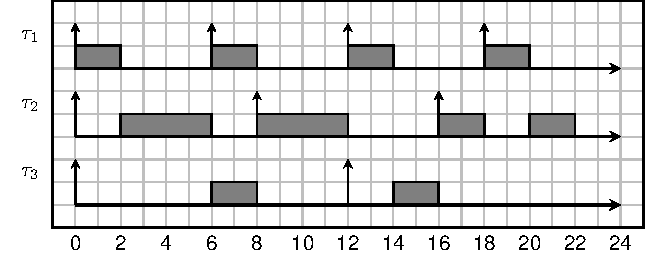
\includegraphics{schedule/edf.pdf}
	\end{figure}
\end{frame}


\begin{frame}[fragile]
	\frametitle{ Application of the previous algorithm }
	\begin{figure}
		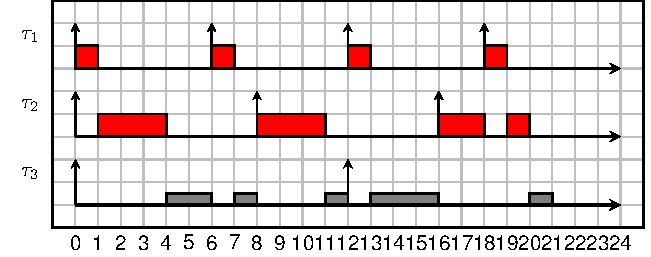
\includegraphics{schedule/offline_algo.pdf}
	\end{figure}
	
\end{frame}

\subsection{Online Algorithms}

\begin{frame}
	\frametitle{Online algorithms}
	\begin{block}{Dynamic frequency scaling for FLASH}
		If we can still complete the task with the worst case time execution before the deadline. Then we lower the frequency. 
	\end{block}
	\begin{block}{Dynamic CCM SRAM allocation}
		\begin{itemize}
			\item Divide the CCM into slots
			\item Before executing copy task instructions in the CCM slot
			\item the worst case execution time is equal to the CCM execution time with the associated memcopy
			
		\end{itemize}
		$\Rightarrow$ Changes in the scheduling algorithm: mutex, blocking, non-preemptive tasks $\ldots$

	\end{block}
\end{frame}

\begin{frame}
	\frametitle{STM32G}
	\begin{block}{Different execution modes}
		\begin{itemize}
			\item Range 1 mode (normal) : normal execution from 8 to 150 MHz.
			\item Range 1 boost mode : frequency up to 170 MHz, less wait states but higher voltage .
			\item Range 2 low power mode : frequency between 8 and 32 MHz, better consumption in these frequencies.
		\end{itemize}
	\end{block}
	\begin{block}{FLASH cache}
		Allows zero wait states and pre fetch when instructions are in FLASH $\rightarrow$ same results as the CCM.
	\end{block}
\end{frame}


\begin{frame}[plain] % The optional argument 'plain' hides the headline and footline
	\begin{center}
		{\Huge The End}
		
		\bigskip\bigskip % Vertical whitespace
		
		{\LARGE Questions? Comments?}
	\end{center}
\end{frame}

%----------------------------------------------------------------------------------------

\end{document} 